This chapter will focus specifically on control rod cusping effects, which are the focus of this work.  First, a more thorough definition of the problem and motivation for solving it will be presented.  The next section will then present some of the solutions that have been used to minimize the cusping effects in the past, including a simplified decusping model implemented in MPACT itself.  The third section will then discuss some newer methods based on the sublpane CMFD scheme that have recently been implemented in MPACT.  Finally, a new ``sub-ray'' MOC method will be proposed to deal with the cause of the cusping effects on a more fundamental level.

\section{Background}

\begin{figure}[h]
    \centering
    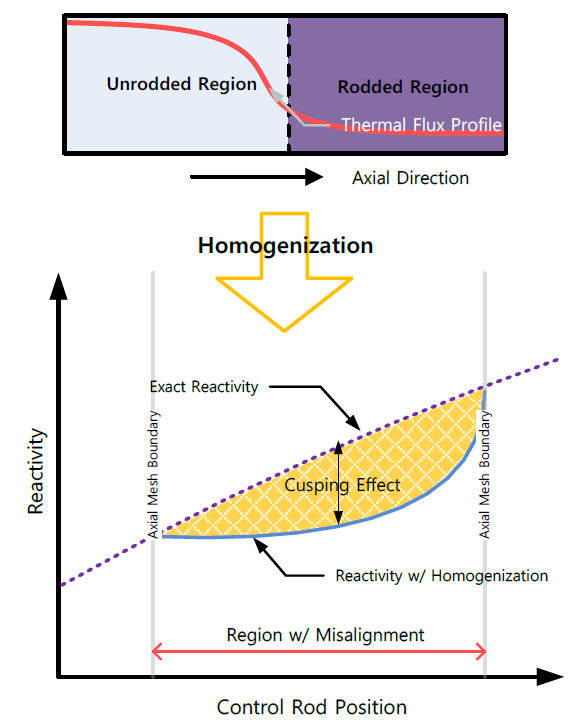
\includegraphics[width=0.4\textwidth]{cusping_effect_Joo.png}
    \caption[Rod Cusping Illustration]{Illustration of Rod ``Cusping'' \cite{ICAPPcontrolRodDecuspingNTRACER}}\label{f:cuspingEffectJoo}
\end{figure}

In Section \ref{s:2d1dErrors}, some potential sources of errors for the 2D/1D scheme were introduced.  One of these was the error introduced by axial homogenization within a 2D MOC plane.  In some cases, this can be done without introducing significant errors.  For example, MPACT often homogenizes components outside the active fuel region, such as the end plugs and gaps at the end of the fuel rods.  However, when strong neutron absorbers, such as control rods, are homogenized axially in active fuel region, this has the effect of introducing absorption in regions where there should be none.  This effect is known as ``cusping,'' \cite{finnemann1977RodCuspingOrigMention} and is illustrated in Figure \ref{f:cuspingEffectJoo}.

In some cases, this is easily handled by setting up an appropriate axial mesh which prevents the need for the homogenization, but this is not always a practical solution.  Throughout the course of an entire cycle of operation (usually about 18 months), several different control banks in the reactor may move to a variety of positions to maintain criticality in the core.  Control rods in a PWR typically have step sizes of approximately 1.5 cm, but a typical MOC plane in MPACT is about 8 cm thick in the active fuel region.  In order to prevent cusping effects for an entire cycle, the user may have to create a very detailed axial mesh to ensure that all the control rod positions used throughout the cycle align with the edge of an MOC plane.  Not only is this tedious for the user, but it also greatly increases the computational burden due to the increased number of MOC planes.  Figure \ref{f:p4cuspingEffects} shows the calculated k-eff as a function of control rod position.  The cusping effects in this figure are further complicated by a heterogeneous rod with AIC and B$_4$C poison regions and a stainless steal tip.  Thus, cusping effects occur not just at the control rod tip, but also at material interfaces throughout the rod.

\section{Decusping Methods History}

Before discussing the recent and proposed methods to address the rod cusping problem, it is useful to provide an overview of past methods.  These will then be used as a comparison for recent work and justification for the proposed work.  First, we will look at some of the ways rod cusping was address in older nodal codes.  Then we will look at the effects in 2D/1D codes and recent work to address them.

\subsection{Nodal Codes}

Control rod decusping methods have been developed for nodal codes for over thirty years now.  Many different methods have been developed over that time frame, making a comprehensive discussion impractical.  However, several different methods will be discussed here to provide some context for how the rod cusping problem was handled in nodal codes.

\subsubsection{Tabulation Methods}

One of the most basic methods of handling the cusping problem was through pre-tabulation of cross-section for the partially rodded node (PRN) \cite{HanSemJooThesis1984}.  For the nodal calculations, node-averaged cross-sections were generated using some higher fidelity method on small portions of the domain.  For the PRN, this calculation could simply be repeated many times for each of the possible rod positions.  However, because of the many positions the control rod could have in a reactor, this required many different cross-sections to be calculated.  Furthermore, these calculations needed to be done on more than a single assembly to obtain acceptable accuracy due to inter-assembly effects \cite{KordSmithThesis1980spatial}.  Others tried using multi-assembly calculations \cite{hoxieThesis1982application} and color sets \cite{khalilThesis1983application} to improve the accuracy of this method.  However, the number of rod possible positions and the size of the problems required to generate accurate homogenized cross-sections made this method impractical at the time, motivating further research into rod decusping methods.

One variation of this method which improved on the runtime used response matrices and node surface currents \cite{chengThesis1981homogenizationResponseMatrix,finckThesis1982homogenizationResponseMatrix}.  For this method, response matrices were tabulated ahead of time based on the surface current boundary conditions.  An iterative process could then be carried out between the global nodal calculation and a local fixed sources calculation.  During each iteration, the surface currents from the global calculation were used to update the homogenized cross-sections in the PRN using the response matrices.  At convergence, the cross-sections in the PRN were calculated from the actual solution boundary conditions, greatly increasing the accuracy of the global solution compared with the simpler cross-section tabulation method.  However, this method still required up-front calculation of the response matrices, which could be expensive for some problems.  Consistency was also not perfectly maintained between the local and global problems, which sometimes resulted in convergence difficulties.

\subsubsection{Polynomial Flux Expansions}

Another early method which sought to improve on the brute-force tabulation method used polynomial expansions of the intra-nodal flux shape in the axial direction \cite{bennewitz1975higher,finnemann1981space}.  Methods such as NEM which are commonly used in nodal codes typically assume some shape to the source and flux inside each node.  For this method, a quadratic shape was assumed and used to flux-volume weight the rodded and unrodded cross-sections to generate homogenized cross-sections for the PRN.  This resulted in a reduction of the cusping errors by about 50\% \cite{KordSmithMastersThesis1979AnalyticNodalMethod}, which was not sufficient for many applications.  Higher order polynomials were also attempted \cite{langenbuch1977coarse}, but the axial shapes these generated were non-physical and sometimes led to oscillations and other numerical problems.

\subsubsection{Collector-Predictor Method}

Joo \cite{HanSemJooThesis1984} focused on developing a method which would address rod decusping using only material compositions and node dimensions, rather than relying on boundary conditions as well.  To do this, he developed an asymptotic method in which the PRN was modeled as two semi-infinite slabs, with one slab being composed of rodded material and the other slab being unrodded material.  A 1D multi-group calculation was then carried out to determine the flux shape around the interface between the two materials.  This flux shape was then used in the homogenization process for the PRN.

This method was found to be inaccurate because the infinite system is not actually a good representation of the flux shape in a reactor.  To improve on this method, Joo developed what is known as the Collector-Predictor Method.  There are two variations to this method.  The first, simpler variation assumes that the first calculation has the tip of the control rod aligned with the boundary between two nodes.  The collector step occurs at the end of the global calculation, collecting the radial transverse leakages and axial boundary currents for the rodded and unrodded nodes which neighbor each other.  Then, rather than performing calculations using semi-infinite slabs as in the previous paragraph, a 1D calculation is instead performed using the information from the collector step.  This predictor step generates a more accurate flux profile around the interface between the rodded and unrodded materials.  Then, when the rod is moved throughout the calculation, it is assumed that this axial flux profile in the vicinity of the rod tip does not change significantly, so the profile can just be shifted with the rod and used in all subsequent cross-section homogenizations.  This method then improved to allow the first calculation to also have a PRN.  Overall, this method significantly improved on previous ones by reducing decusping methods dynamically that converged consistently and did not rely on tabulated values.  Furthermore, because the extra calculations were 1D on a small sub-domain of the problem, the additional computational expense was small.

\subsubsection{Bi-Linear Weighting Method}

Many decusping methods which followed the Collector-Predictor Method focused on improvements to the 1D calculation or boundary condition information to improve accuracy \cite{gehinThesis1992quasi,smith1992enhancementsStudxvickCoreManagementSystem,lee1998CuspingCorrection1DFineMeshFluxProfiles,downar2004PARCStheory}.  However, one significant variation that was developed by Kim and Cho \cite{kim1990BilinearWeighting} is the Bi-Linear Weighting Method.  This method uses the same concept as the Collector-Predictor method, but solves for both the forward and adjoint axial flux shapes.  Both of these shapes are then used in the cross-section homogenization, as shown in Equation \ref{e:bilinearWeighting}.  The use of the adjoint flux in the homogenization process resulted in significant improvements in the accuracy of the nodal calculations.
\begin{equation}\label{e:bilinearWeighting}
\overline{\Sigma} = \frac{\intop \phi\left(z\right) \phi^*\left(z\right) \Sigma\left(z\right) dz}{\intop \phi\left(z\right) \phi^*\left(z\right) dz}\ .
\end{equation}

\subsubsection{Nodal Expansion Method Modification}\label{sss:NEMmod}

Another method which calculates axial flux profiles to improve homogenization is a modified form of NEM \cite{de2012NEMmodification,martinez1999NEMmodOrig}.  To improve the accuracy of nodal calculations, NEM assumes a quartic polynomial for the intra-nodal flux shape to calculate interface currents.  For the PRN, this quartic shape can can also be used to calculate improved cross-sections.  This is convenient because this axial profile must already be calculated when using NEM, so the only additional calculation is to integrate the shape over the rodded and unrodded region and use the result to homogenize the cross-sections.  Because Legendre polynomials are used for the flux expansion, these integrals can be calculated analytically, resulting in negligible increase in computational cost.

\subsubsection{Equivalent-Node Method}

The Equivalent-Node Method \cite{dall2002nodeEquivalenceDecusping} attempts to calculate the PRN cross-sections as if the PRN were modeled as two separate nodes: one fully rodded and one fully unrodded.  This method sets up two different diffusion problems for the PRN: on with a single region and one with two regions.  This is done in combination with NEM for each of the spatial moments being calculated.  The cross-sections in the case of the single region (homogenized cross-sections) are formulated in terms weighting factors multiplied by the heterogeneous cross-sections.  It is then enforced that the integral of the reaction rates for the one- and two-region problems are equal.  This preserves the reaction rates of the two-node problem in the homogenized problem and provides correction factors for the higher-order spatial moments.  Solving these equations produces accurate, smoothly varying homogenized cross-sections.

\subsubsection{Inverse Spectral Index Method}

With increased computing power, interest grew in performing full-core calculations with finer spatial discretizations by perform nodal calculations using homogenized pins instead of homogenized assemblies or quarter assemblies.  However, with the smaller spatial regions, the radial leakages become more important than before, causing many of the older rod decusping methods to become inaccurate.  In 2004, Yamamoto developed the Inverse Spectral Index (ISI) method to address rod cusping for a pin-by-pin nodal calculation \cite{yamamoto2004pinByPinNodalDecusping}.

To develop this method, it must be noted that if the axial leakage is small compared to the radial leakage, the flux spectrum in a cell will be similar for an assembly calculation or a full-core calculation.  When performing assembly calculations to generate homogenized cross-sections, one quantity which can be tabulated is the spectral index, defined as the ratio of the fast flux to the thermal flux in a pin.  Because the fast flux is smoothly varying across the core compared to the thermal flux, it can be accurately approximated using the PRN's neighbor nodes.  The spectral index from the assembly calculations, which explicitly modeled the rodded and unrodded regions, can then be used with the fast flux to calculate the thermal flux.  A flux-volume weighting is then used to average the rodded and unrodded cross-sections for the following iteration.  Because the fast flux is affected by the PRN cross-sections, iterations are performed to converge the flux and cross-sections together

\subsubsection{CIAMA Nodal Method}

Recently, a new nodal method known as Channel-wise Intrinsic Axial Mesh Adaptation (CIAMA) has been developed \cite{yu2015CIAMArodDecusping,lu2015CIAMAintro}.  This method eliminates all rod cusping effects implicitly by eliminating the traditional constraint of other nodal methods: all nodes must be homogeneous.  With this requirement removed, partially inserted control rods can be handled implicitly by the method, without need for any auxiliary calculations or corrections.

To do this, a sub-plane--like scheme is employed in the NEM formulation.  As with a traditional NEM formulation, the nodes are coupled through transverse leakage terms.  However, within each node, a refined heterogeneous axial mesh is used.  The transverse leakage terms are still calculated on the coarse mesh with a quadratic polynomial fit.  For each node, this polynomial can simply be integrated over the height of the sub-nodes to determine the sub-node leakage source.  Because the inter-node coupling is done on the coarse mesh, the axial sub-mesh can be unique for each node.  This allows the method to implicitly handle axial heterogeneities with minimal increases in runtime.

\subsection{2D/1D Codes}\label{ss:2d1d-old-decusping-methods}

Unfortunately, moving away from nodal methods to higher fidelity transport codes does not eliminate the rod cusping problem, as shown in Figure \ref{f:p4cuspingEffects}.  There have not been as many 2D/1D codes as there have been nodal codes, but each of them still had to contend with this problem.  This section will discuss some of the different 2D/1D codes that have been developed and how the rod cusping problem was dealt with in each of them.

\begin{figure}[h]
    \centering
    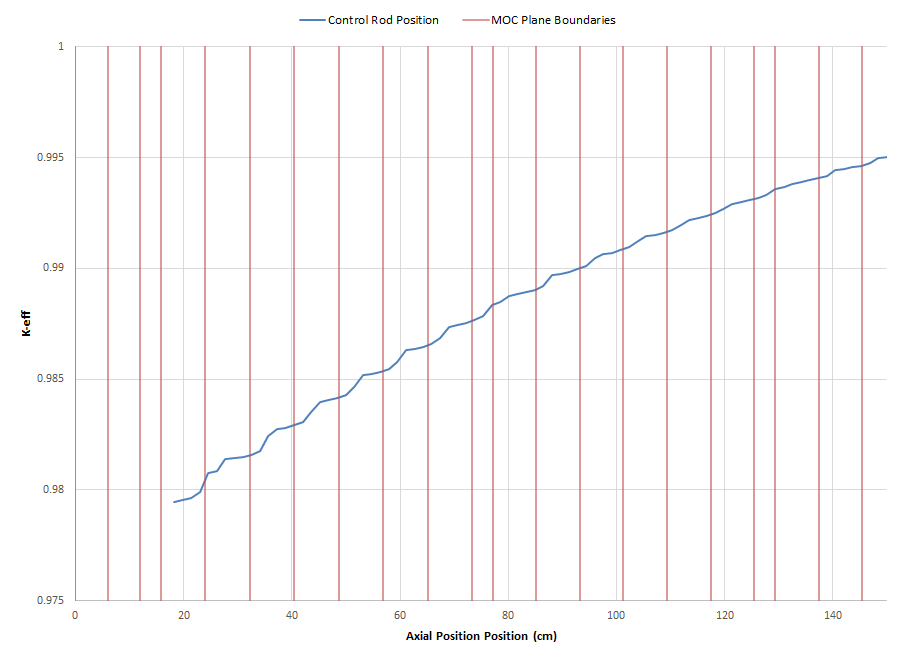
\includegraphics[width=0.8\textwidth]{p4cuspingEffects.png}
    \caption[Rod Cusping in MPACT]{Control Rod Cusping Effects in MPACT for 3x3 Assembly}\label{f:p4cuspingEffects}
\end{figure}

\subsubsection{Neighbor Spectral Index Method}

The code CRX-2K \cite{cho2015CRX2d1dFusionDecusping} uses the 2D/1D fusion method to perform LWR simulations.  To address the rod cusping problem in this code, a modified version of the ISI method is applied, called the Neighbor Spectral Index (NSI) method.  The NSI method uses the same methodology as the ISI with one modification.  Because the 2D/1D fusion method does not require standalone calculations to generate homogenized cross-sections, the spectral index must be calculated on-the-fly during the 2D/1D iteration.  To do this, the neighboring node above the PRN is used to obtain a rodded spectral index, and the neighboring node below the PRN is used to obtain an unrodded spectral index.  These two indexes are then used with the rodded and unrodded cross-sections and volume fractions to obtain homogenized cross-sections for the PRN.  This method causes significant improvements over other decusping methods and requires negligible additional computation since the fluxes are stored for every region already.

\subsubsection{Sub-Plane Decusping}\label{sss:ntracerDecusping}

Another 2D/1D code is nTRACER, which is under active development by Seoul National University \cite{RyuBEAVRSnTRACER2015}.  To address rod cusping effects in nTRACER, Jung and Joo developed a more general method than the polynomial correction method used by MPACT \cite{ICAPPcontrolRodDecuspingNTRACER}.  This method pre-generates correction factors at the start of a simulation, rather than relying on hard-coded corrections.  To do this, the assembly that will have a partially inserted control rod is identified, and a single-plane 3x3 assembly problem is set up using the partially-rodded assembly and its neighbors.  The radial and axial cusping effects are then determined separately.  First, the radial cusping effects are determined by performing 2D MOC calculations on the 3x3 sub-domain with the rod fully inserted and fully withdrawn.  This provides radial flux profiles in the rodded assembly for both rodded and unrodded regions, as well as current coupling coefficients for CMFD for the rodded and unrodded CMFD nodes.  Once this is done, the rod is simulated at positions of 25\%, 50\%, and 75\% withdrawn from the plane.  To reduce runtime, these calculations are done using only 3D sub-plane CMFD, using the heterogeneous rodded and unrodded cross-section for the appropriate sub-planes.  This generates axial flux profiles for the full MOC plane for each of the possible rod positions.  During the full-core 2D/1D calculation, these axial flux profiles are then used to generate improved homogenized cross-sections for the MOC calculation using equation.
\begin{equation}\label{e:nTRACERdecusping}
\overline{\Sigma_i} = \frac{\phi_{rad,i}^R \phi_{ax,i}^R \Sigma_i^R h^R + \phi_{rad,i}^U \phi_{ax,i}^U \Sigma_i^U h^U}{\phi_{rad,i}^R \phi_{ax,i}^R h^R + \phi_{rad,i}^U \phi_{ax,i}^U h^U}\ .
\end{equation}

\subsubsection{Polynomial Corrections}\label{sss:polynomialDecusping}

MPACT currently uses a simple polynomial correction to the volume fractions used to homogenize the control rod \cite{MC2015_VCS_Cycle_Depletion}.  To develop this method, a 3x3 assembly was set up with a control rod in the center assembly.  This problem was simulated with the rod tip at nine different positions in the plane.  These simulations were then repeated, but with the axial mesh refined so the rod tip aligned with a plane boundary.  The k$_{eff}$ differences between the two sets of simulations were fitted with a sixth-order polynomial which is used in MPACT to reduce the volume fraction of the control rod by an appropriate amount to offset the cusping effects.  This process was repeated for different control rod materials such as AIC, B$_4$C, and Tungsten, since each material has unique cross-sections.  This method has the advantages of being simple to implement and requiring no increase in computational requirements.  However, the results obtained from this decusping method are tied to the control rod material and reactor model used to develop the corrections, limiting its usefulness to a small subset of reactors.

\section{Recent Decusping Methods Development}

This section discusses two new decusping treatments added to MPACT.  These methods rely on the sub-plane scheme described in section \ref{ss:2d1d-3dcmfd}.  The first method only treats the axial cusping effects, while the second method extends the first by also treating the radial decusping effects.

\subsection{Sub-plane Decusping}

In section \ref{ss:2d1d-3dcmfd}, the sub-plane scheme was introduced as a means of coarsening the 2D/1D axial mesh to improve runtime while maintaining accuracy.  However, one negative consequence of using the sub-plane scheme is that it increases the likelihood of partially inserted rods being present since there are fewer, thicker MOC planes.  To address this, two modifications were made to the sub-plane scheme to minimize cusping effects.  The resulting method shares some similarities with the one employed by nTRACER discussed in section \ref{sss:ntracerDecusping}.  However, this method is built directly into the 2D/1D iteration scheme, requiring no additional MOC calculations to inform the decusping calculations.

The first modification that was made was to modify the cross-sections used for the sub-plane CMFD and axial SP$_3$ calculations.  In the most basic form of the sub-plane scheme, the same cross-sections and radial coupling coefficients are used for all sub-planes in each MOC plane.  To use sub-plane as a decusping method, the requirement for constant cross-sections was removed.  Thus, when Equation \ref{e:CMFDhomogTerms} is applied, explicit rodded or unrodded cross-sections are used for the cross-section homogenization in each sub-plane, rather than a single homogenized cross-section being using in all sub-planes.  This allows the CMFD and axial solvers to capture the sharp flux gradients that occur around the edge of the control rods.

In order to improve the MOC calculations as well, the CMFD flux projection described in Equation \ref{e:CMFDscaling} is extended to also include a cross-section projection for the partially rodded pin cells.  This is done using Equation \ref{e:nTRACERdecusping} with $\phi_{rad,i}^R = \phi_{rad,i}^U$.  This allows the 2D MOC calculations to also capture some of the axial effects of the partially inserted rod.

\subsection{Auxiliary 1D Collision Probabilities}

While the sub-plane decusping method is better than none, it captures only the axial effects of the partially inserted rod.  To also capture the radial effects, an additional radial calculation is needed to obtain radial flux profiles for the rodded and un-rodded regions.  In MPACT, this is done using a 1D Collision Probabilities (CP) solver.

\begin{figure}[h]
  \centering
  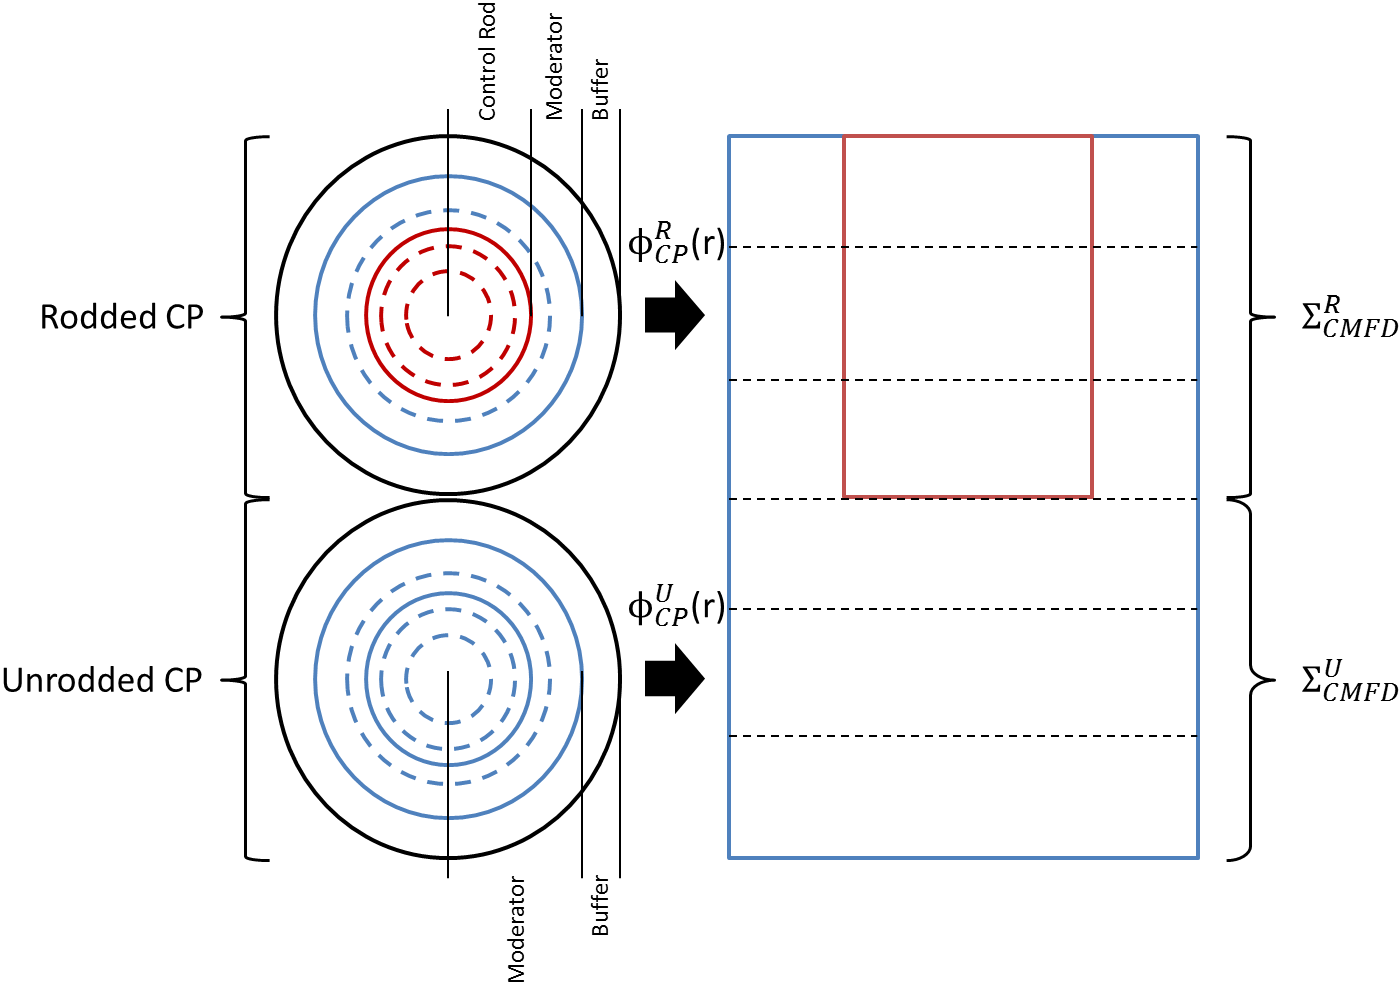
\includegraphics[width=\textwidth]{CPdecusp.png}
  \caption[Collision Probabilities Decusping]{Illustration of 1D Collision Probabilities rod decusping method}\label{f:CPdecusp}
\end{figure}

After the CMFD homogenization, but prior to the calculation itself, a 1D CP kernel is solved for the rodded and un-rodded regions to obtain a radial flux profile.  This calculation uses the MOC cross-sections in each radial zone, along with a buffer region that consists of the eight neighboring CMFD cells homogenized together.  These profiles are normalized so that the volume-average of each profile is exactly unity.  These profiles are then used with the sub-plane CMFD flux and material cross-sections to calculate improved homogenized cross-sections, as shown in Equation \ref{e:CPMxs}.  Homogenizing the cross-sections in this way allows CMFD to capture both axial and radial effects of the partially inserted rod with negligible increase in computational expense.  This process is illustrated in Figure \ref{f:CPdecusp}.
\begin{equation}\label{e:CPMxs}
\Sigma_{g,i}=\frac{1}{\phi_{g,i}V_i}\sum_{r=1}^{N_{rings}} \Sigma_{g,r} \phi_{CMFD,g,i} \phi_{CP,g,r} V_r\ .
\end{equation}

After the CMFD calculation, the MOC cross-sections must be modified as with the sub-plane decusping.  This is done using by using Equation \ref{e:nTRACERdecusping} directly, where the radial flux terms are the projected MOC fluxes and the axial flux terms are the results of the sub-plane CMFD calculation that used the CP-homogenized cross-sections.  The projection of the CMFD flux to the MOC mesh is unchanged from the standard sub-plane scheme.  The CMFD calculation flow when using 1D CP is shown in Figure \ref{f:1dcpm-flowchart}

\begin{figure}
  \centering
  \begin{tikzpicture}[node distance=2cm]

% Start
\node (start) [startstop] {Start};

% CMFD
\node (homog) [process, right of=start, xshift=2.0cm] {Homogenize cross-sections and flux; Calculate $\tilde{D}$};
\node (1dcpm) [process, below of=start, yshift=-0.5cm] {1D CP calculations};
\node (homogCP) [process, right of=1dcpm, xshift=2.0cm] {Re-homogenize cross-sections in partially rodded pin cells};
\node (iterCheck) [decision, below of=homogCP, yshift=-1.5cm] {First iteration?};
\node (firstIter) [process, below of=iterCheck, xshift=-2.5cm, yshift=-1.0cm] {Set $\hat{D}=0$};
\node (laterIter) [process, below of=iterCheck, xshift=2.5cm, yshift=-1.0cm] {Calculate $\hat{D}$};
\node (matrix) [process, below of=firstIter, xshift=2.5cm] {Set up CMFD matrix};
\node (3DCMFD) [process, below of=matrix] {3D CMFD calculation};
\node (proj) [process, below of=3DCMFD] {Scale MOC flux with CMFD flux};
\node (projCP) [process, below of=proj] {Homogenize partially rodded MOC cross-sections};

% Stop
\node (stop) [startstop, right of=projCP, xshift=2.0cm] {Stop};

% Basic Arrows
\draw [arrow] (start) -- (homog);
\draw [arrow] (1dcpm) -- (homogCP);
\draw [arrow] (homogCP) -- (iterCheck);
\draw [arrow] (matrix) -- (3DCMFD);
\draw [arrow] (3DCMFD) -- (proj);
\draw [arrow] (proj) -- (projCP);
\draw [arrow] (projCP) -- (stop);

% Fancy Arrows
\draw [arrow] (homog) |- ([yshift=-0.75cm]start.south) -| (1dcpm);
\draw [arrow] (iterCheck) -| node[anchor=south] {yes} (firstIter);
\draw [arrow] (iterCheck) -| node[anchor=south] {no} (laterIter);
\draw [arrow] (firstIter) |- (matrix);
\draw [arrow] (laterIter) |- (matrix);

\end{tikzpicture}
  \caption[Stuff]{Calculation flow for CMFD calculation in MPACT with 1D CP decusping treatment}\label{f:1dcpm-flowchart}
\end{figure}